
\subsection{بهبودیافته}
این الگوریتم ابتدا هدف و موقعیت شروع را توسط یک خط مستقیم به هم متصل می کند. سپس فهرستی از مراکز، که نقاطی روی خط هستند که برخورد کردن به آن ها ممنوع می باشد را  ایجاد می کند. برای هر مرکز، دایره‌ای به شعاع معین \lr{r} 
در اطراف این نقاط می‌سازد، و سپس مختصات محل ها ی برخورد این دایره ها را با خط پیدا می کند به عنوان نمونه شکل 
\ref{improved}
ر ادر نظر بگیرید . سپس با انتخاب هر یک از این جفت ها به عنوان نقطه شروع و هدف محلی، با استفاده از آستانه
$\epsilon$
بررسی می کند که آیا هدف محلی 
\lr{E}
و شروع محلی بعدی 
\lr{ I} 
به یکدیگر نزدیک هستند یا خیر. اگر نزدیک باشند، هدف محلی فعلی به هدف محلی بعدی تغییر می کند، یعنی برنامه ریز باید مسیری را از 
\lr{D }
به
\lr{K}
، همانطور که در شکل نشان داده شده است، برنامه ریزی کند. پس از انجام این کار، الگوریتم با استفاده از الگوریتم 
\lr{A*}
، مسیرهای موضعی را در اطراف همه جفت های 
\lr{(D,E)} 
و 
\lr{(D,K)}
مسیریابی می کند.  رد نهایت مسیری حاصل می شود که بخشی از آن شامل خطی راست است که کواه ترین مسیر است و موانع با استفاده از الگوریتم
\lr{ A*}
دور زده می شوند .

\begin{figure}[h]
	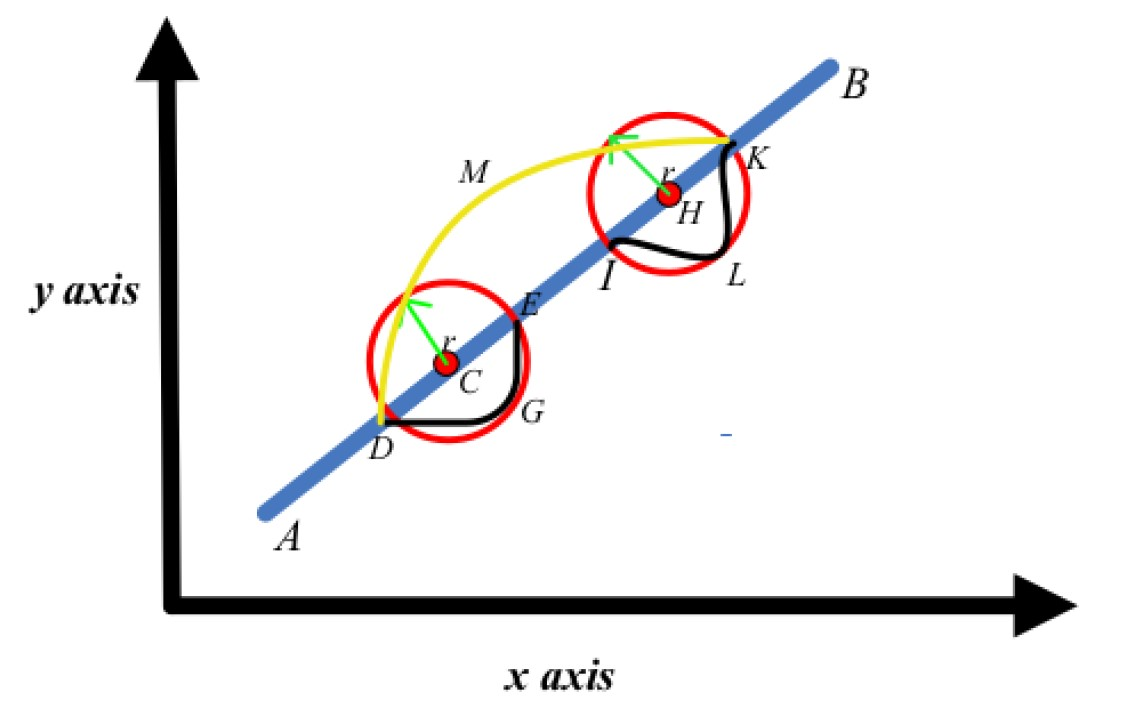
\includegraphics[scale=0.4]{improved}
	\centering
	\caption{ شیوه کار  \lr{A*}بهبود یافته}
	\cite{paliwal2023survey}
	\label{improved}
\end{figure}